	\section{Fonctionnement général}
	Lorsque je suis arrivé sur le projet, une partie de la conception était déjà réalisée, le fonctionnement général de la plateforme. Cette conception permet de répondre aux attentes du problème, tout en permettant le maximum d'évolutions facilement.
	
	\subsection{Le fichier Walkthrough}\label{wt}
		Le fichier Walkthrough est un fichier qui sera fourni par la personne en charge des tests, c'est un fichier au format Excel qui contient les informations de chacune des variables à tester. Il contient ainsi un très grand nombre de colonnes, bien que seul une partie des colonnes nous intéresse, certaines colonnes ont été fournies par le fournisseur du plugin, d'autres colonnes sont ajoutées dans le seul but de la génération de tests automatiques par \textit{GreenT}. Voici les colonnes intéressantes : 

		\begin{description} 
			\item[Nom de la variable] Le nom de la variable testé : il existe un nom court et un nom long.
			\item[Informations aidant à la conversion des données] Certains \textit{devices} tel que le debugger ne fonctionne qu'avec des valeurs Hexadécimales. À la charge de \textit{GreenT} de convertir ces données vers des valeurs physiques exploitables par le testeur
			\item[Nécessité d'un test automatique] un \texttt{GreenTTest} ne sera généré que si la colonne vaut \textit{Yes}.
			\item[Statut du test] Nous éditerons cette colonne afin de reporter le statut du test.
			\item[Precondition (cf section \ref{stim})] Contient un scénario d'initialisation du \textit{workbench} : tension de départ, lancement du debugger, \ldots
			\item[Scénario de stimulation (cf section \ref{stim})] Contient un ou plusieurs scénarios de stimulations
			\item[ExpectedBehavior (cf section \ref{expectedBehavior})] Contient une expression évaluant les variables ayant été enregistrées durant la stimulation : \textit{GreenT} devra vérifier que cette expression est correct à toute instant de la stimulation.
			\item[Variable à enregistrer (cf section \ref{expectedBehavior})] Contient les variables devont être enregistrées durant un scénario, en plus des variables présentes dans l'expected behavior.
			\item[Alias locaux (cf section \ref{alias})] Ce sont des alias déclarés uniquement pour le test courant.
			\item[Informations du test (cf section \ref{report})] Plusieurs colonnes tel que la sévérité, le responsable du test, les commentaires, \ldots
		\end{description}

		\begin{figure}[H]
			\centering
			\includegraphics[width=18.5cm]{contents/images/walkthrough.png}
			\caption{Aperçu d'un fichier Walkthrough}
		\end{figure}

	\subsection{Fonctionnalités principales}
	Le développement de \textit{GreenT} va inclure un certain nombre de fonctionnalités attendues par le client et indispensable à son fonctionnement. D'autres fonctionnalités pourront apparaître plus tard en fonction des besoins.

	Les interactions entre les différents modules de \textit{GreenT} sont schématisées figure \ref{fig:generalDig}

	\subsubsection{Parsing et Génération}\label{generation}
	Le but premier de la plateforme est d'effectuer des tests automatiques, il est ainsi indispensable d'avoir un système d'automatisation.

	Pour cela, nous allons avoir un parser : il analysera un certain type de fichier\footnote{Nous ne commencerons qu'avec le Walkthrough pour débuter, mais dans le futur nous pourrions avoir des fichiers XML, des bases de données, \ldots} et en retirera pour chaque test, le scénario de pré condition, les différents scénarios de stimulations, leurs \textit{Expected Behavior}, les données qui devront être enregistrées ainsi que les différentes données du test\footnote{Responsable du test, sévérité, commentaires, nom de la variable, \ldots}.

	Une fois toutes ces données acquises, il les transmettra à un générateur qui sera en charge d'écrire les fichiers Java de chaque test, tous seront organisés dans un dossier temporaire avec un dossier par test. Le \texttt{TestManager} pourra ensuite traiter ces données.

	\subsubsection{Résolution des alias}\label{alias}
		Les devices ont des fonctionnements différents pour leurs variables internes, le HIL\footnote{Hardware in the loop} par exemple utilise des adresses de base de données, alors que le debugger fonctionne avec des valeurs Hexadécimales permettant d'accéder directement à des cases RAM.

		Il est donc indispensable de fournir au client une approche permettant de masquer ces différences, et le risque d'erreur en écrivant une adresse, pour cela nous avons pensé un système d'alias : un alias possède un nom qui permet de le lier une valeur sur le device à un nom de variable, le client n'aura ensuite plus qu'à travailler avec des noms clairs et explicites.

		Il y a deux types d'alias : ceux qui sont accessibles en écriture, et ceux accessibles en lecture, on pourra donc effectuer des actions différentes en fonction du type d'alias.

		\begin{figure}[H]
			\centering
			\includegraphics[width=13cm]{contents/images/classAlias.png}
			\caption{Diagramme de classes des Alias}
		\end{figure}
		Les alias en écriture sont répartis en deux types : les alias HIL et les alias Debugger, car ils n'ont pas les même méthodes : il est possible de faire un set hexadécimal sur un debugger, contrairement à un HIL qui lui permet d'effectuer un set électrique. 

	\subsubsection{Stimulation} \label{stim}
		Afin de tester une variable du plugin, les développeurs vont utiliser des alias présents sur un équipement\footnote{De l'anglais \textit{Device}} : actuellement, un HIL ou un debugger, prochainement nous pourrions en utiliser d'autres que ces deux derniers.

		Le spécifieur va rédiger des scénarios de stimulation, ceci afin de mettre le contrôleur dans certaines conditions. Son but sera ensuite de vérifier que ces variables restent cohérentes vis-à-vis du scénario effectué. 

		Un scénario particulier doit être spécifié : une pré condition qui a pour but d'initialiser les \textit{devices} et certains alias afin d'avoir un état de stimulation qui soit cohérent et identique à chaque lancement du scénario. Ce scénario sera effectué avant le lancement de chacun des scénarios de stimulation.

	\subsubsection{Les traces et leurs évaluations}\label{expectedBehavior}
	Lorsqu'un scénario de stimulation s'exécute, un certain nombre de variables doivent être enregistrées : ces variables sont stockées sous la forme d'une trace au format CSV, qui pourra plus tard être représentée sous forme de courbe. 

	Une fois que la trace est complète, il est nécessaire de l'évaluer : le spécifieur a fournis une \textit{Expected Behavior} détaillant dans quel cas le test est correct, ainsi cette expression va être transformée en arbre logique afin de l'évaluer à tout instant T de la trace. Une fonctionnalité de couverture de tests sera fourni afin de s'assurer qu'un test de sévérité \textit{High} est correctement spécifié.

	\subsubsection{Le TestManager}\label{testManager}
	Le TestManager est le chef d'orchestre de \textit{GreenT}, il a donc un certain nombre de responsabilités. 

	Il va d'abord organiser les différents tests en un concept que nous avons appelé \textit{Bundle} : afin de limiter le temps d'exécution qui atteindra plusieurs dizaines d'heures, il est intéressant de regrouper les tests possédant les mêmes scénarios de stimulations et les mêmes pré conditions. Seules leur \textit{Expected Behavior} changent, mais celles-ci pourront être évaluées sur la même Trace.

	Une fois les tests organisés en Bundle, il va les compiler et les donner à un \texttt{WorkbenchManager} : toujours pour une raison d'optimisation, il sera intéressant de pouvoir exécuter les enregistrements sur plusieurs bancs simultanément, pour cela le \texttt{TestManager} sera capable de savoir quels bancs peuvent être utilisés et pourra distribuer ses bundles en fonction. 

	Chaque WorkbenchManager sera en charge d'exécuter le code généré plus tôt et dialoguera en réseau avec son banc, une fois l'exécution terminée, il obtiendra une trace qui pourra être évaluée.

	Afin d'être le plus souple possible, il existe plusieurs modes d'exécution du \texttt{TestManager} : 
	\begin{description}
		\item[Check only] Essaye de parser les différents fichiers, et vérifie que ceux-ci ne comportent aucune erreur de grammaire, d'alias introuvable, d'écriture sur un alias en lecture seule etc...
		\item[Parse and generate jar tests] Parse les fichiers et génère des jars exécutables pour chacun des tests
		\item[Parse and genere bundles] Parse les fichiers et génère des jars exécutables répartis en bundle
		\item[Parse and execute] Parse les fichiers, génère les jars pour les bundles et les exécute : c'est le mode << classique >>.
		\item[Restart test execution] Redémarre une exécution qui se serait mal terminée.
	\end{description}
	\subsubsection{Production de rapport détaillé}\label{report}
	La plateforme aura en charge la production d'un rapport détaillé pour chaque test. Ce rapport contiendra un certain nombre d'informations, et permettra au testeur de comprendre pourquoi le test n'est pas passé. Voici les informations que contiendra ce rapport : 

	\begin{itemize}
		\item Nom du test, de la variable à tester
		\item Nom du responsable du test
		\item Sévérité du test
		\item Pourcentage de branches de l'expectedBehavior renvoyant faux\footnote{Test << Rouge >>}, n'ayant pas pu être testé\footnote{Test << Gris >>} et étant correct\footnote{Test Vert}
		\item Le testeur aura à sa disposition les expressions concernés par un résultat Rouge ou Gris.
		\item Les colonnes utiles du \textit{Walkthrough}
	\end{itemize}

	Le format du rapport détaillé n'a pas encore été définis, mais cela pourrait être des fichiers textes, avec pour évolution une possibilité de le faire sous format Web avec affichage des courbes de trace par exemple.

	\subsubsection{Mise à jour du Walkthrough}
	Une fois un test exécuté, un résultat sera mis dans le fichier Excel, en fonction de la sévérité du test. En effet, un test \textit{High} ne devra comporter aucune branche non testée contrairement à un test \textit{Low} par exemple.
	
	\subsubsection{Schéma de fonctionnement global}
		\begin{figure}[H]
			\centering
			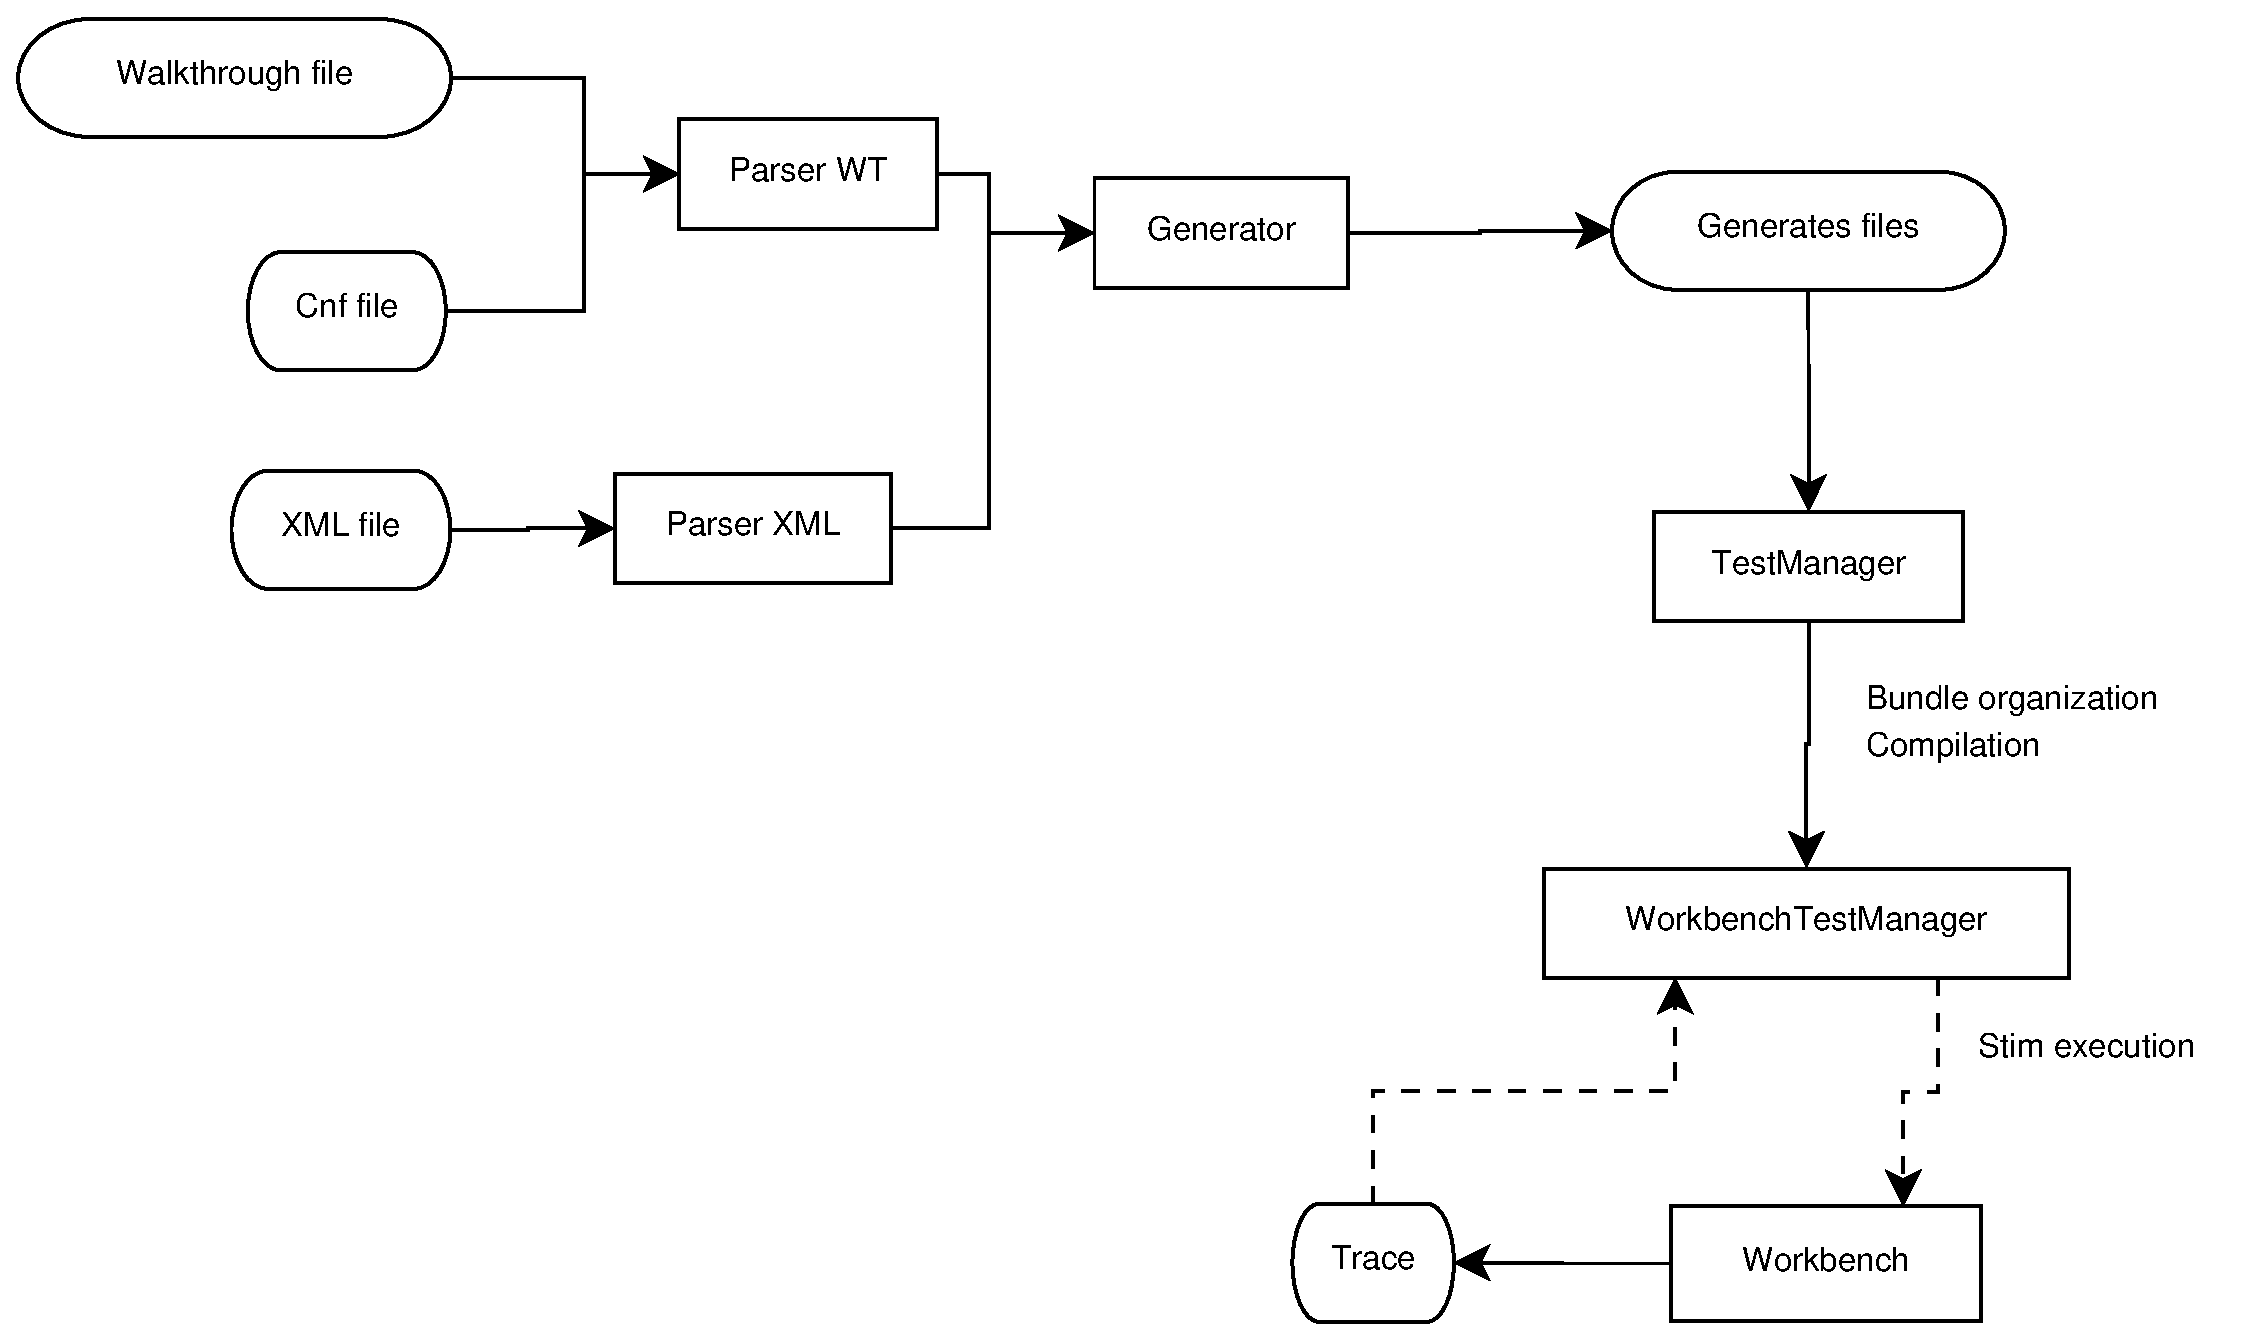
\includegraphics[width=15.5cm]{contents/images/generalDiag.eps}
			\caption{Fonctionnement général du parser \textit{GreenT}}
			\label{fig:generalDig}
		\end{figure}
		Dans ce schéma nous pouvons voir les différents modules détaillés précédemment : un type de parser prend en entrée un fichier, qu'il analyse, génère les fichiers Java, les donnes au \texttt{TestManager}, qui les organise en \textit{Bundle}, les compiles, donne les binaires au \texttt{WorkbenchTestManager}, qui dialogue directement avec le banc, une fois le bundle exécuté, celui-ci retourne la trace. Il ne reste plus qu'a l'analyser et prononcer un verdict.\\
		Dans des objets ovales sont représentés des fichiers, les carrés représentent des modules de la plateforme et les flèches en pointillés un transfert réseau.

	Pour ma part, je me suis occupé de la partie du parser, du générateur, et j'ai aidé à la conception du système d'évaluation et d'analyses des traces.
